\documentclass[journal, a4paper]{IEEEtran}
\usepackage{graphicx}   % Written by David Carlisle and Sebastian Rahtz
\usepackage{url}        % Written by Donald Arseneau
\usepackage{amsmath}    % From the American Mathematical Society
\usepackage{hyperref}
\usepackage[backend=biber,style=numeric,sorting=none]{biblatex}
\addbibresource{refs.bib}
% Your document starts here!
\begin{document}

% Define document title and author
	\title{Report Template with Notebook}
	\author{FirstName LastName
	\thanks{Advisor:~Spicklemire, Stephen J.}}
	\markboth{Physical Measurements: PHYS 415, report 1}{}
	\maketitle

% Write abstract here
\begin{abstract}
(\textit{Note: please make a copy of this template before editing!}) The short abstract (50-80 words) is intended to give the reader a {\it brief} overview of the work and the relevant results. 
\end{abstract}

% Each section begins with a \section{title} command
\section{Introduction}
	% \PARstart{}{} creates a tall first letter for this first paragraph
	\PARstart{T}{his} section describes the physical context of the investigation, and research question to be answered and some insight into the motivation for the investigation.
% Theory and Background
\section{Theory and Background}
	% LaTeX takes complete care of your document layout ...
	This is where you provide references to background information or theory that the reader might need to understand your project. This could include textbook references or other
    resources. Anything you don't work out here, but that you need for to complete
    the analysis, should be referenced.
	% ... but you can insert a line break manually with two backslashes, if needed: \\

\section{Experimental apparatus and set up, Data Acquisition, and Data}
	This is where you describe the experiment. What are the uncertainties in the raw data? What does the reader need to know to evaluate the quality and validity of your results? 
	You should give data in tabular form, if it's pretty limited, or 
    provide an online reference for your data (e.g., think google sheets, or plotly).
    This is {\it not} a procedure from a lab report, but an explanation that a
    competent researcher could use to reproduce your results. Only non-obvious details
    need to be included, especially things that may have required some trial and error to 
    get good results. In other words, don't make a colleague make the same mistakes
    you did to get good results, tell them the tricky bits of how you did it, but 
    they don't need to know that you plugged in the light sensor, or turned on the laser.
    
\section{Analysis}
	How did you analyze the data to answer the research question? Explain. Evaluate the uncertainty in the results. Explain.

\section{Discussion}
	What did you learn from the data? How was the result significant? How does the result relate to the original research question? What 
    future improvements can you suggest, and why?
    
\section{Format}
	The report can be written in \LaTeX{} or Microsoft Word, but \LaTeX{} is definitely preferred.Its appearance should be as close to this document as possible to achieve consistency between papers.

	% You can cite a book or paper by using \cite{reference}.
	% The references will be defined at the end of this .tex file in the bibliography
	References should be saved in the {\tt refs.bib} file and should be cited by name (example: ``... as shown by Einstein, 1905 \parencite{einstein}, ...''). The BibLaTeX system will automatically create the references list based on which references are cited in the text \parencite{dirac}.

	References should be of academic character and should be published and accessible.
	Your advisor can answer your questions regarding literature research.
	You must cite all used sources.	Examples of good references include text books and scientific journals or conference proceedings.	If possible, citing internet pages should be avoided.In particular, Wikipedia is \emph{not} an appropriate reference in academic reports.
	Avoiding references in languages other than English is recommended.

	% You can reference tables and figure by using the \ref{label} command. Each table and figure needs to have a UNIQUE label.
	Figures and tables should be labeled and numbered, such as in Table~\ref{tab:simParameters} and Fig.~\ref{fig:tf_plot}. \url{http://www.google.com}

	% This is how you define a table: the [!hbt] means that LaTeX is forced (by the !) to place the table exactly here (by h), or if that doesnt work because of a pagebreak or so, it tries to place the table to the bottom of the page (by b) or the top (by t).
	\begin{table}[!hbt]
		% Center the table
		\begin{center}
		% Title of the table
		\caption{Simulation Parameters}
		\label{tab:simParameters}
		% Table itself: here we have two columns which are centered and have lines to the left, right and in the middle: |c|c|
		\begin{tabular}{|c|c|}
			% To create a horizontal line, type \hline
			\hline
			% To end a column type &
			% For a linebreak type \\
			Information message length & $k=16000$ bit \\
			\hline
			Radio segment size & $b=160$ bit \\
			\hline
			Rate of component codes & $R_{cc}=1/3$\\
			\hline
			Polynomial of component encoders & $[1 , 33/37 , 25/37]_8$\\
			\hline
		\end{tabular}
		\end{center}
	\end{table}

% If you have questions about how to write mathematical formulas in LaTeX, please read a LaTeX book or the 'Not So Short Introduction to LaTeX': tobi.oetiker.ch/lshort/lshort.pdf

% This is how you include a pdf figure in your document. LaTeX only accepts EPS or TIFF files.
	\begin{figure}[!hbt]
		% Center the figure.
		\begin{center}
		% Include the pdf file, scale it such that it's width equals the column width. You can also put width=8cm for example...
		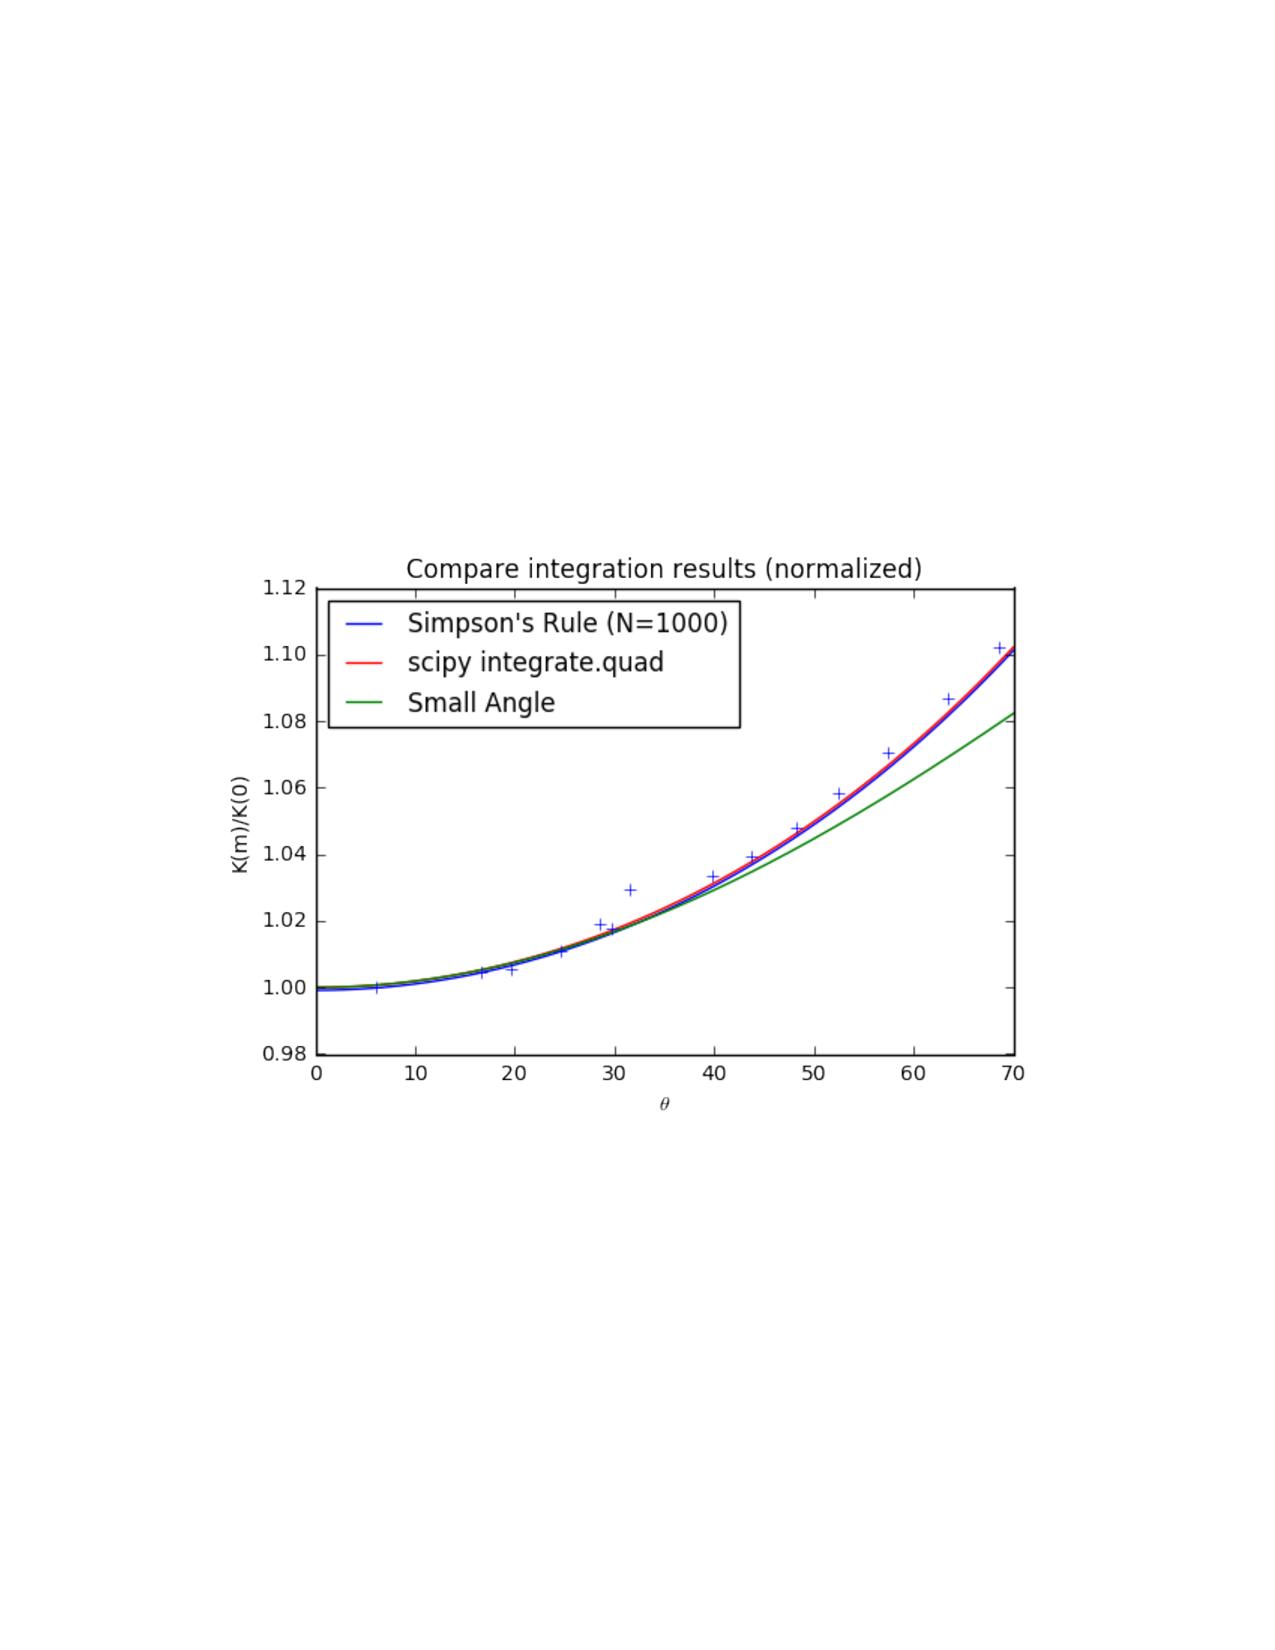
\includegraphics[width=\columnwidth]{pendulum}
		% Create a subtitle for the figure.
		\caption{Comparison of experimental results and theoretical prediction.}
		% Define the label of the figure. It's good to use 'fig:title', so you know that the label belongs to a figure.
		\label{fig:tf_plot}
		\end{center}
	\end{figure}

% Now we need a bibliography:
\printbibliography[title={References}]

% Your document ends here!
\end{document}